% Requires graphicx. Copy the PDF files alongside this snippet or adjust paths.
\begin{figure*}[t]
\centering
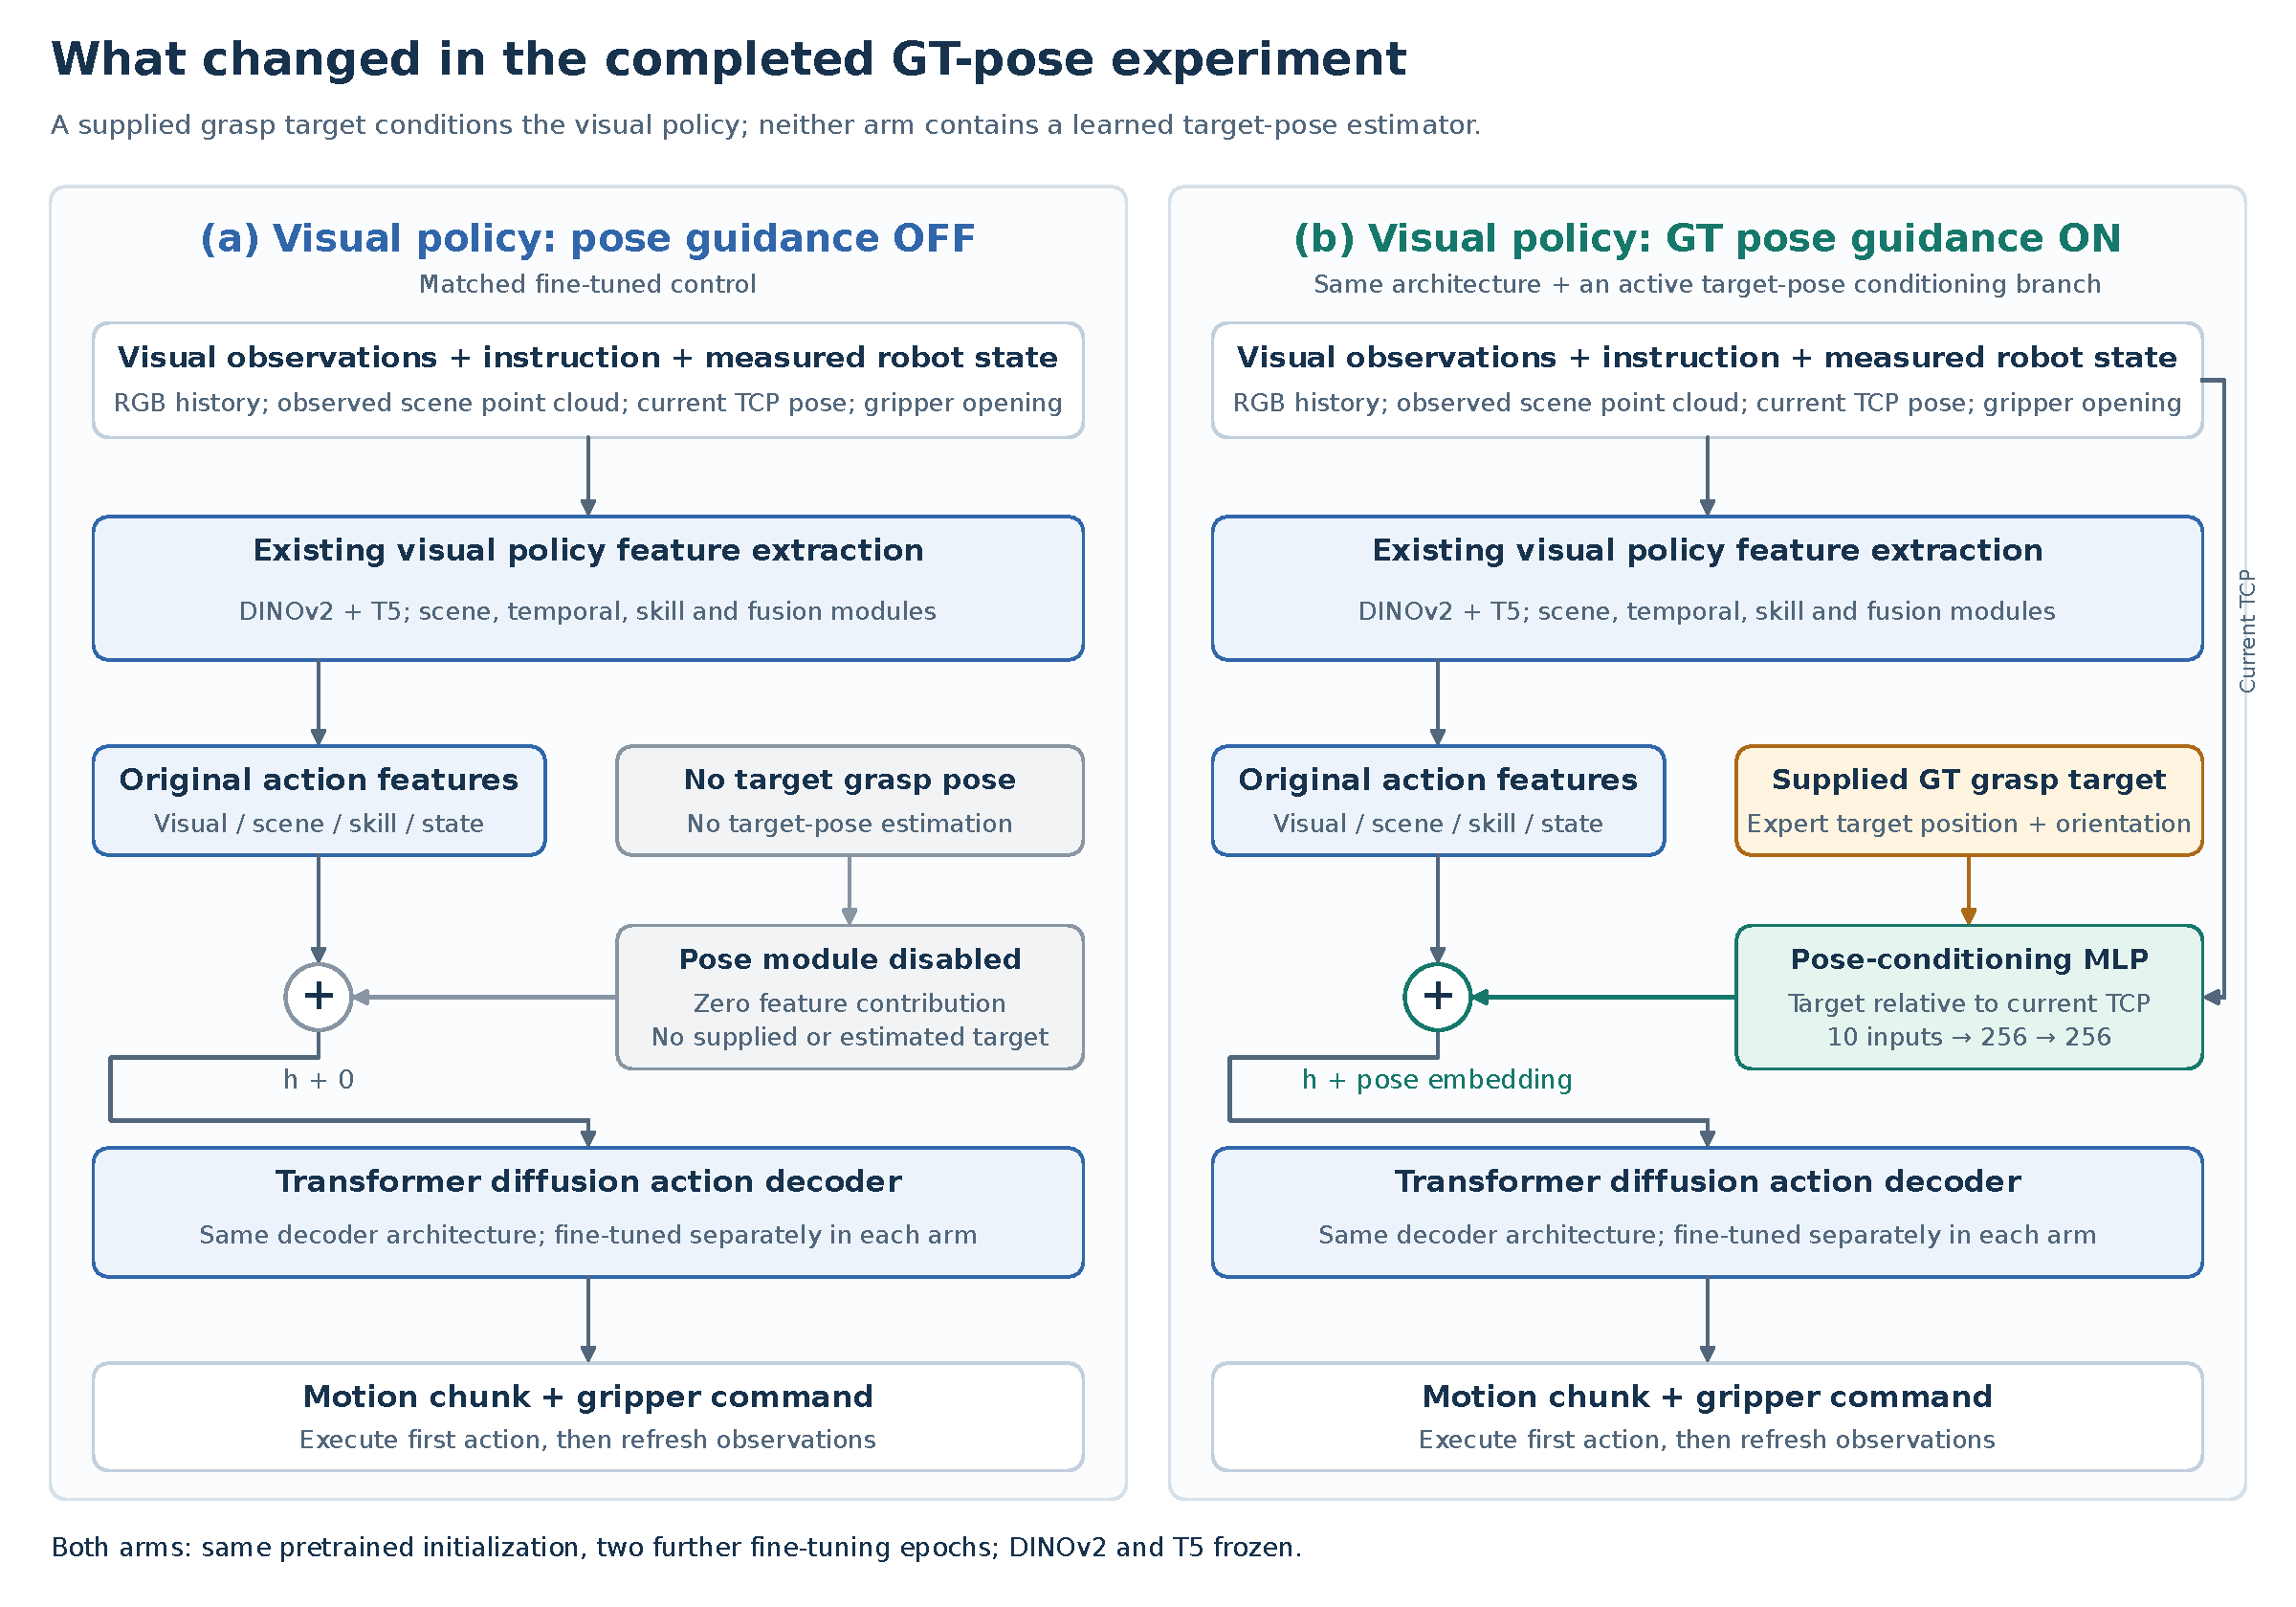
\includegraphics[width=\textwidth]{architecture/evaluated_pose_off_vs_gt_pose.pdf}
\caption{Evaluated comparison of target-pose guidance in the original visual policy.
Both arms retain RGB history, observed scene point clouds, language, measured current TCP pose,
and gripper opening. The control masks the pose module's contribution to zero. The GT arm
embeds a supplied expert-reference grasp TCP target relative to the measured current TCP and
adds the embedding to the original action features. The diffusion decoder architecture is
the same; learned weights are fine-tuned separately from the same pretrained initialization.
No learned target-pose estimator or separate action-overriding controller is used in either arm.
The first-grasp reference target is static and supplied through the episode where available.
Auxiliary heads and losses are omitted for readability.}
\label{fig:evaluated-pose-guidance}
\end{figure*}

\begin{figure*}[t]
\centering
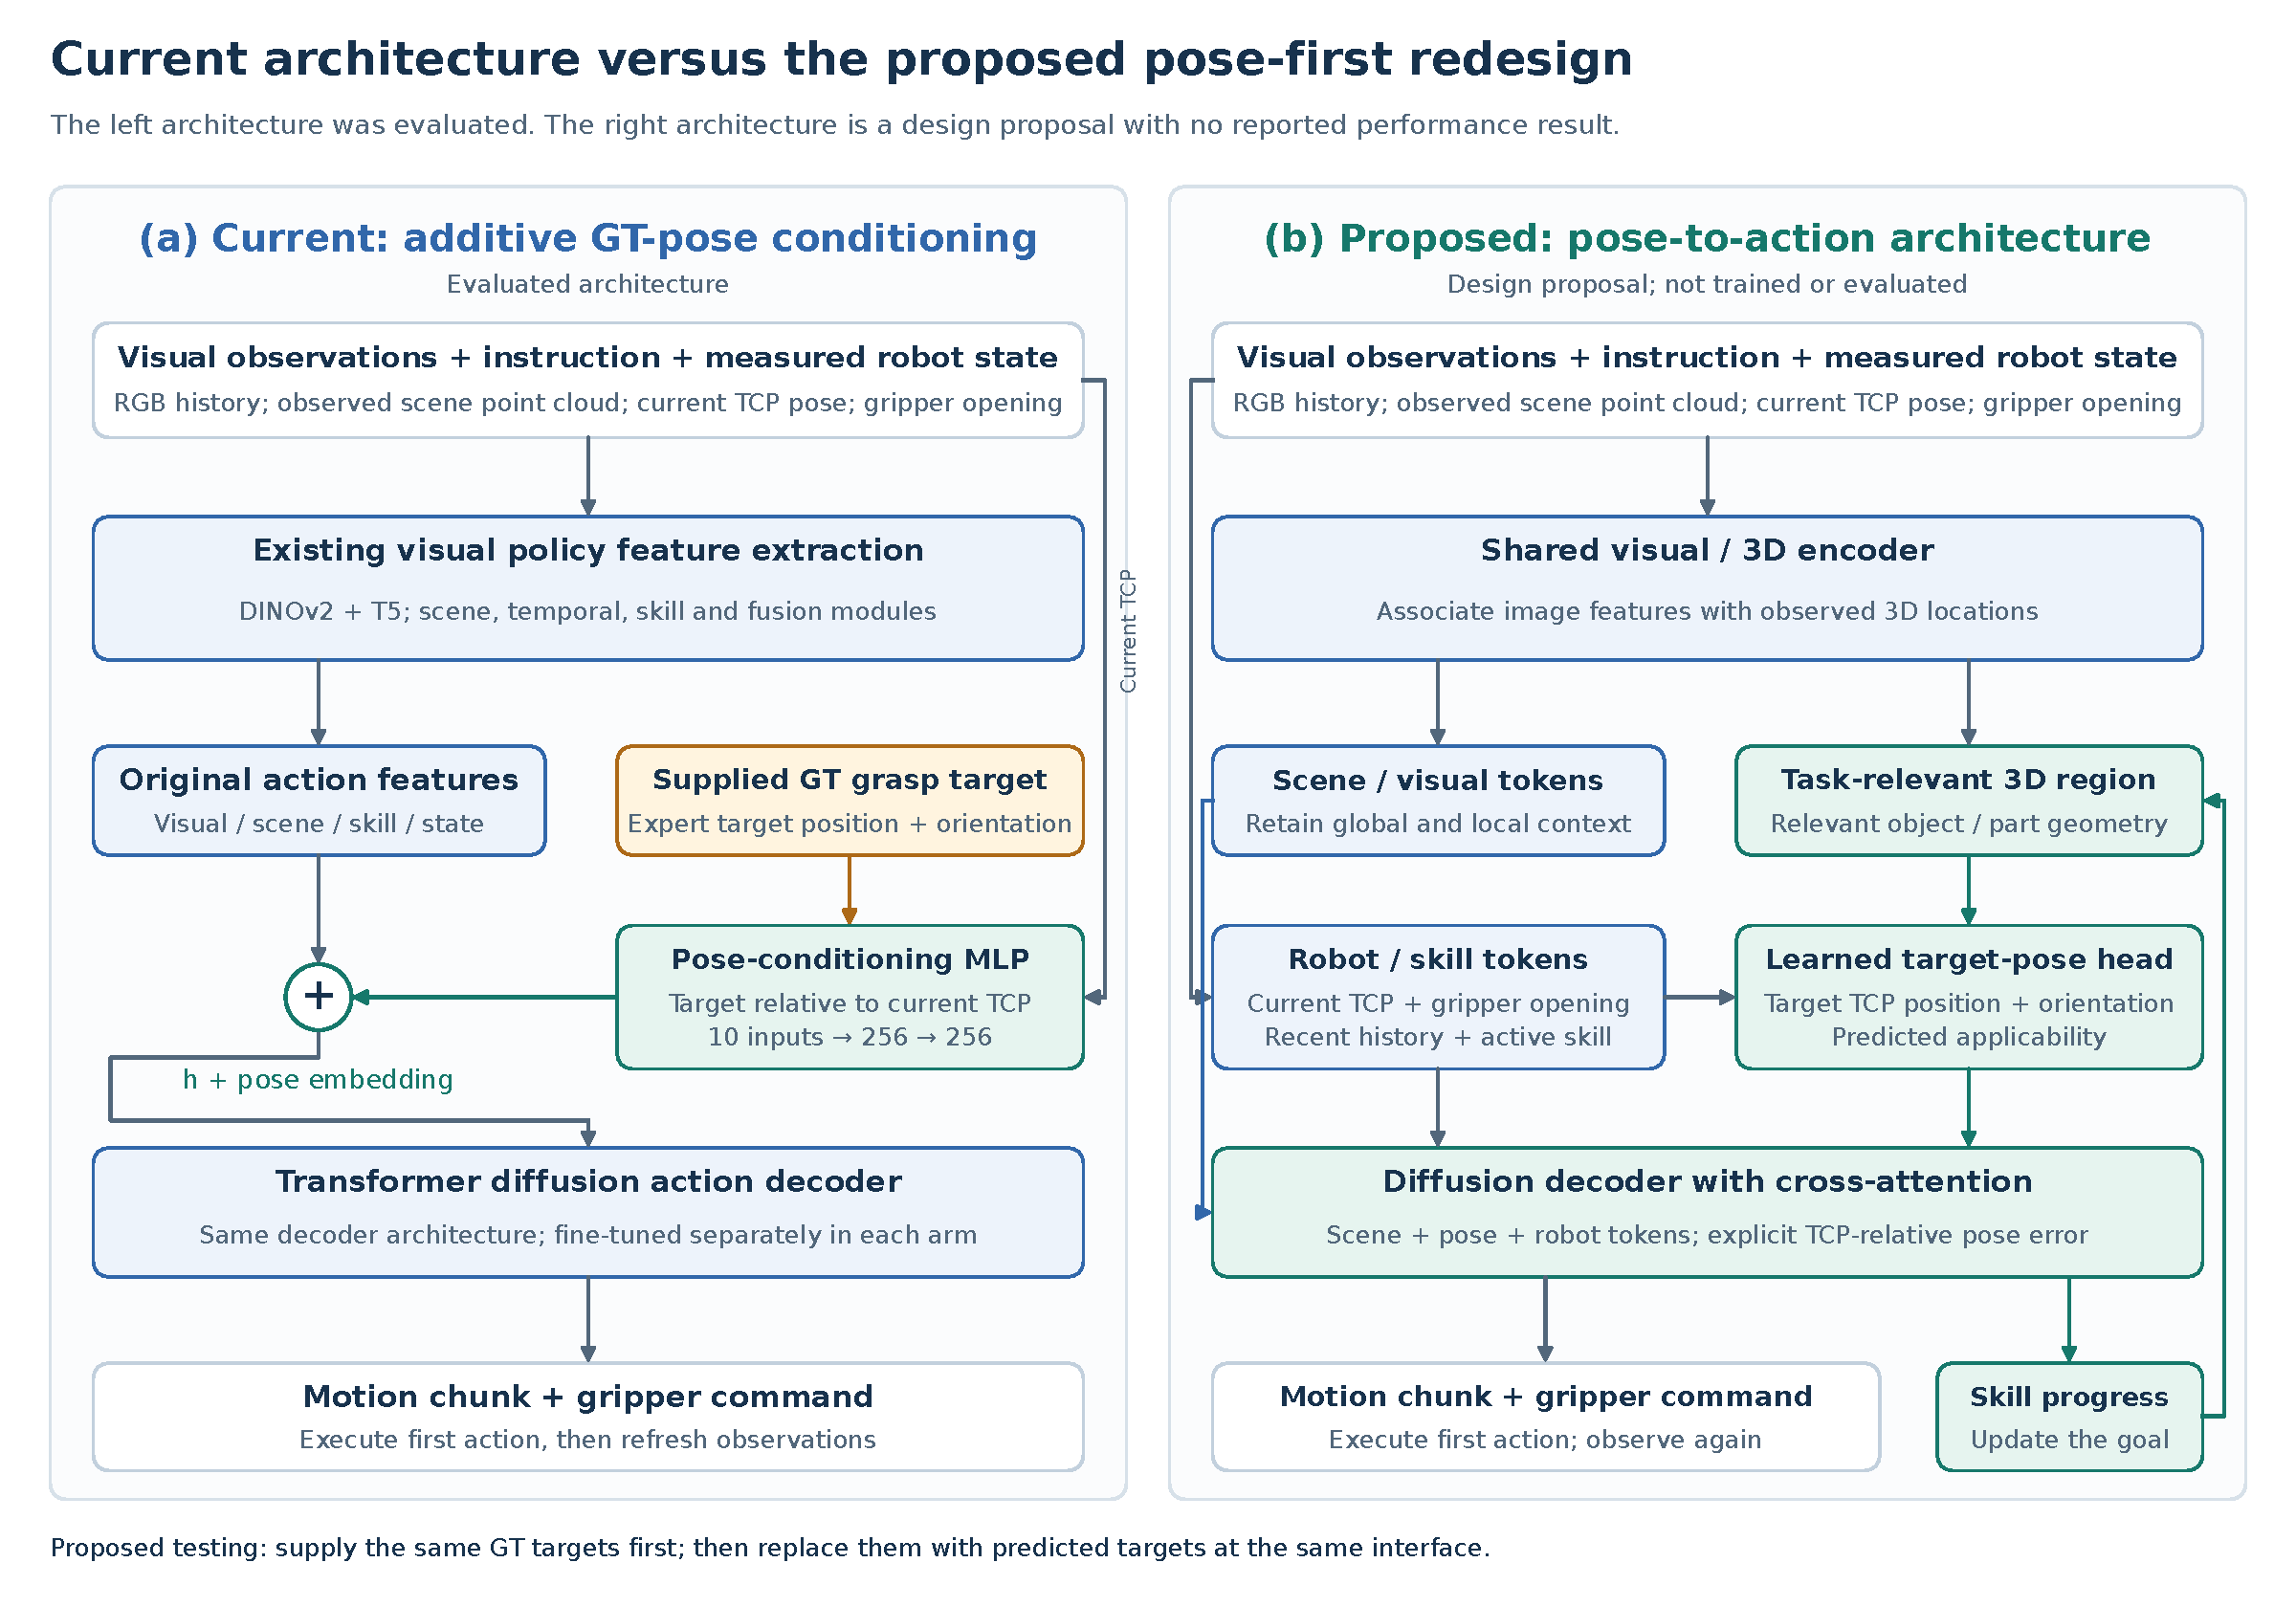
\includegraphics[width=\textwidth]{current_vs_proposed_pose_first.pdf}
\caption{Current additive GT-pose conditioning versus a proposed pose-first redesign.
The proposal associates RGB features with observed 3D locations, grounds a task-relevant
region, predicts a target TCP pose and applicability, and preserves scene, pose, and robot
context as tokens for a cross-attention diffusion actor. A progress head uses the goal,
scene, and robot state to support skill transitions. Its arrows are a conceptual dependency
diagram rather than a finalized software graph. A controlled experiment can substitute the
same supplied GT targets at the proposed pose interface before evaluating learned targets.
Later-skill goals require additional supervision. The proposed architecture has not been
trained or evaluated, and no performance improvement is claimed.}
\label{fig:proposed-pose-first}
\end{figure*}
